\documentclass{article}
\usepackage{tikz}
\usetikzlibrary{patterns}
\usepackage{subcaption}
\usepackage[margin=0.5in]{geometry}

\begin{document}

\begin{figure}[ht]
    \centering
    \begin{subfigure}{0.32\textwidth}
        \centering
        \resizebox{\textwidth}{!}{\input{non_boundary_ok_v2_a.tex}}
        \caption{Full Lattice}
    \end{subfigure}
    \hfill
    \begin{subfigure}{0.32\textwidth}
        \centering
        \resizebox{\textwidth}{!}{\input{non_boundary_ok_v2_b.tex}}
        \caption{$\mathcal{L}
    \end{subfigure}
    \hfill
    \begin{subfigure}{0.32\textwidth}
        \centering
        \resizebox{\textwidth}{!}{\input{non_boundary_ok_v2_c.tex}}
        \caption{$\mathcal{L}
    \end{subfigure}
    \vspace{0.5cm}
    \begin{subfigure}{0.32\textwidth}
        \centering
        \resizebox{\textwidth}{!}{\input{non_boundary_ok_v2_d.tex}}
        \caption{$\mathcal{L}
    \end{subfigure}
    \hfill
    \begin{subfigure}{0.32\textwidth}
        \centering
        \resizebox{\textwidth}{!}{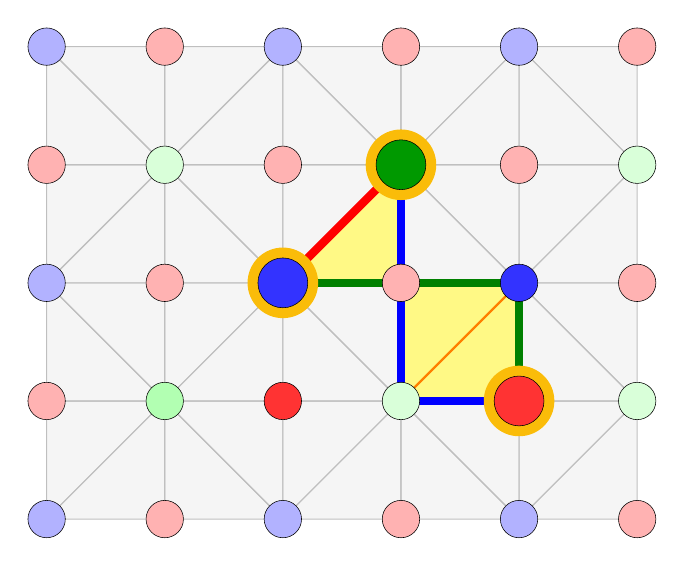
\begin{tikzpicture}[scale=1.5]
    \filldraw[fill=gray!15, draw=gray!50, , fill opacity=0.5] (-2,-2) -- (-1,-2) -- (-1,-1) -- cycle;
    \filldraw[fill=gray!15, draw=gray!50, , fill opacity=0.5] (-2,-2) -- (-2,-1) -- (-1,-1) -- cycle;
    \filldraw[fill=gray!15, draw=gray!50, , fill opacity=0.5] (-2,0) -- (-2,-1) -- (-1,-1) -- cycle;
    \filldraw[fill=gray!15, draw=gray!50, , fill opacity=0.5] (-2,0) -- (-1,0) -- (-1,-1) -- cycle;
    \filldraw[fill=gray!15, draw=gray!50, , fill opacity=0.5] (-2,0) -- (-1,0) -- (-1,1) -- cycle;
    \filldraw[fill=gray!15, draw=gray!50, , fill opacity=0.5] (-2,0) -- (-2,1) -- (-1,1) -- cycle;
    \filldraw[fill=gray!15, draw=gray!50, , fill opacity=0.5] (-2,2) -- (-2,1) -- (-1,1) -- cycle;
    \filldraw[fill=gray!15, draw=gray!50, , fill opacity=0.5] (-2,2) -- (-1,2) -- (-1,1) -- cycle;
    \filldraw[fill=gray!15, draw=gray!50, , fill opacity=0.5] (0,-2) -- (-1,-2) -- (-1,-1) -- cycle;
    \filldraw[fill=gray!15, draw=gray!50, , fill opacity=0.5] (0,-2) -- (0,-1) -- (-1,-1) -- cycle;
    \filldraw[fill=gray!15, draw=gray!50, , fill opacity=0.5] (0,0) -- (0,-1) -- (-1,-1) -- cycle;
    \filldraw[fill=gray!15, draw=gray!50, , fill opacity=0.5] (0,0) -- (-1,0) -- (-1,-1) -- cycle;
    \filldraw[fill=gray!15, draw=gray!50, , fill opacity=0.5] (0,0) -- (-1,0) -- (-1,1) -- cycle;
    \filldraw[fill=gray!15, draw=gray!50, , fill opacity=0.5] (0,0) -- (0,1) -- (-1,1) -- cycle;
    \filldraw[fill=gray!15, draw=gray!50, , fill opacity=0.5] (0,2) -- (0,1) -- (-1,1) -- cycle;
    \filldraw[fill=gray!15, draw=gray!50, , fill opacity=0.5] (0,2) -- (-1,2) -- (-1,1) -- cycle;
    \filldraw[fill=gray!15, draw=gray!50, , fill opacity=0.5] (0,-2) -- (1,-2) -- (1,-1) -- cycle;
    \filldraw[fill=gray!15, draw=gray!50, , fill opacity=0.5] (0,-2) -- (0,-1) -- (1,-1) -- cycle;
    \filldraw[fill=gray!15, draw=gray!50, , fill opacity=0.5] (0,0) -- (0,-1) -- (1,-1) -- cycle;
    \filldraw[fill=gray!15, draw=gray!50, , fill opacity=0.5] (0,0) -- (1,0) -- (1,-1) -- cycle;
    \filldraw[fill=yellow!60, draw=orange, thick, fill opacity=0.8] (0,0) -- (1,0) -- (1,1) -- cycle;
    \filldraw[fill=gray!15, draw=gray!50, , fill opacity=0.5] (0,0) -- (0,1) -- (1,1) -- cycle;
    \filldraw[fill=gray!15, draw=gray!50, , fill opacity=0.5] (0,2) -- (0,1) -- (1,1) -- cycle;
    \filldraw[fill=gray!15, draw=gray!50, , fill opacity=0.5] (0,2) -- (1,2) -- (1,1) -- cycle;
    \filldraw[fill=gray!15, draw=gray!50, , fill opacity=0.5] (2,-2) -- (1,-2) -- (1,-1) -- cycle;
    \filldraw[fill=gray!15, draw=gray!50, , fill opacity=0.5] (2,-2) -- (2,-1) -- (1,-1) -- cycle;
    \filldraw[fill=yellow!60, draw=orange, thick, fill opacity=0.8] (2,0) -- (2,-1) -- (1,-1) -- cycle;
    \filldraw[fill=yellow!60, draw=orange, thick, fill opacity=0.8] (2,0) -- (1,0) -- (1,-1) -- cycle;
    \filldraw[fill=gray!15, draw=gray!50, , fill opacity=0.5] (2,0) -- (1,0) -- (1,1) -- cycle;
    \filldraw[fill=gray!15, draw=gray!50, , fill opacity=0.5] (2,0) -- (2,1) -- (1,1) -- cycle;
    \filldraw[fill=gray!15, draw=gray!50, , fill opacity=0.5] (2,2) -- (2,1) -- (1,1) -- cycle;
    \filldraw[fill=gray!15, draw=gray!50, , fill opacity=0.5] (2,2) -- (1,2) -- (1,1) -- cycle;
    \filldraw[fill=gray!15, draw=gray!50, , fill opacity=0.5] (2,-2) -- (3,-2) -- (3,-1) -- cycle;
    \filldraw[fill=gray!15, draw=gray!50, , fill opacity=0.5] (2,-2) -- (2,-1) -- (3,-1) -- cycle;
    \filldraw[fill=gray!15, draw=gray!50, , fill opacity=0.5] (2,0) -- (2,-1) -- (3,-1) -- cycle;
    \filldraw[fill=gray!15, draw=gray!50, , fill opacity=0.5] (2,0) -- (3,0) -- (3,-1) -- cycle;
    \filldraw[fill=gray!15, draw=gray!50, , fill opacity=0.5] (2,0) -- (3,0) -- (3,1) -- cycle;
    \filldraw[fill=gray!15, draw=gray!50, , fill opacity=0.5] (2,0) -- (2,1) -- (3,1) -- cycle;
    \filldraw[fill=gray!15, draw=gray!50, , fill opacity=0.5] (2,2) -- (2,1) -- (3,1) -- cycle;
    \filldraw[fill=gray!15, draw=gray!50, , fill opacity=0.5] (2,2) -- (3,2) -- (3,1) -- cycle;
    \draw[blue, line width=3pt] (2,-1) -- (1,-1);
    \draw[blue, line width=3pt] (1,-1) -- (1,0);
    \draw[blue, line width=3pt] (1,0) -- (1,1);
    \draw[green!50!black, line width=3pt] (2,-1) -- (2,0);
    \draw[green!50!black, line width=3pt] (2,0) -- (1,0);
    \draw[green!50!black, line width=3pt] (1,0) -- (0,0);
    \draw[red, line width=3pt] (1,1) -- (0,0);
    \filldraw[fill=blue!30, draw=black, very thin] (-2, -2) circle (4.5pt);
    \filldraw[fill=red!30, draw=black, very thin] (-2, -1) circle (4.5pt);
    \filldraw[fill=blue!30, draw=black, very thin] (-2, 0) circle (4.5pt);
    \filldraw[fill=red!30, draw=black, very thin] (-2, 1) circle (4.5pt);
    \filldraw[fill=blue!30, draw=black, very thin] (-2, 2) circle (4.5pt);
    \filldraw[fill=red!30, draw=black, very thin] (-1, -2) circle (4.5pt);
    \filldraw[fill=green!30, draw=black, very thin] (-1, -1) circle (4.5pt);
    \filldraw[fill=red!30, draw=black, very thin] (-1, 0) circle (4.5pt);
    \filldraw[fill=green!15, draw=black, very thin] (-1, 1) circle (4.5pt);
    \filldraw[fill=red!30, draw=black, very thin] (-1, 2) circle (4.5pt);
    \filldraw[fill=blue!30, draw=black, very thin] (0, -2) circle (4.5pt);
    \filldraw[fill=red!80, draw=black, very thin] (0, -1) circle (4.5pt);
    \filldraw[fill=yellow!50!orange, draw=none] (0, 0) circle (8.5pt);
    \filldraw[fill=blue!80, draw=black, very thin] (0, 0) circle (6pt);
    \filldraw[fill=red!30, draw=black, very thin] (0, 1) circle (4.5pt);
    \filldraw[fill=blue!30, draw=black, very thin] (0, 2) circle (4.5pt);
    \filldraw[fill=red!30, draw=black, very thin] (1, -2) circle (4.5pt);
    \filldraw[fill=green!15, draw=black, very thin] (1, -1) circle (4.5pt);
    \filldraw[fill=red!30, draw=black, very thin] (1, 0) circle (4.5pt);
    \filldraw[fill=yellow!50!orange, draw=none] (1, 1) circle (8.5pt);
    \filldraw[fill=green!60!black, draw=black, very thin] (1, 1) circle (6pt);
    \filldraw[fill=red!30, draw=black, very thin] (1, 2) circle (4.5pt);
    \filldraw[fill=blue!30, draw=black, very thin] (2, -2) circle (4.5pt);
    \filldraw[fill=yellow!50!orange, draw=none] (2, -1) circle (8.5pt);
    \filldraw[fill=red!80, draw=black, very thin] (2, -1) circle (6pt);
    \filldraw[fill=blue!80, draw=black, very thin] (2, 0) circle (4.5pt);
    \filldraw[fill=red!30, draw=black, very thin] (2, 1) circle (4.5pt);
    \filldraw[fill=blue!30, draw=black, very thin] (2, 2) circle (4.5pt);
    \filldraw[fill=red!30, draw=black, very thin] (3, -2) circle (4.5pt);
    \filldraw[fill=green!15, draw=black, very thin] (3, -1) circle (4.5pt);
    \filldraw[fill=red!30, draw=black, very thin] (3, 0) circle (4.5pt);
    \filldraw[fill=green!15, draw=black, very thin] (3, 1) circle (4.5pt);
    \filldraw[fill=red!30, draw=black, very thin] (3, 2) circle (4.5pt);
\end{tikzpicture}
}
        \caption{Projection Merge (Success)}
    \end{subfigure}
    \hfill
    \begin{subfigure}{0.32\textwidth}
        \centering
        \resizebox{\textwidth}{!}{\input{non_boundary_ok_v2_f.tex}}
        \caption{Restriction (Success)}
    \end{subfigure}
    
    \vspace{0.5cm}
    \caption{Full Lattice}
\end{figure}

\end{document}